\section{Problem 2}

We describe the pseudocode for the problem in \Cref{alg:iterjarvis}. Intuitively we iteratively apply Jarvis March algorithm and remove the current convex hull layer from the current set of points. Once this is done we binary search for query point $q$.

\begin{algorithm}
\caption{Convex Layering \label{alg:iterjarvis}}
\begin{algorithmic}[1]
\STATE $S\ \leftarrow$ Set of randomly allocated points
\STATE $ConvLayers\ \leftarrow\ \phi$ (Dynamically alloted 2D array to store layers).
\STATE $l = 0$
\WHILE {S is not empty}
	\STATE Run Jarvis March on $S$. Let the convex hull computed be $\mathcal H^S$
	\STATE $ConvLayers[k]\ \leftarrow\ \mathcal H^S$ 
	\STATE $S\ \leftarrow\ S\setminus \mathcal H^S$, $k++$
\ENDWHILE
\STATE Return $ConvLayers$ representing the $k$ convex layers.
\STATE Run a binary search on $ConvLayers$ with query point $q$ and output the depth accordingly.
\end {algorithmic}
\end{algorithm}


\subsection{Time and Space Complexity}
Time taken to compute the convex hull layers is clearly $O(\sum_{i\in [k]}(|ConvLayers[i]|.n))$ which is $O(n^2)$ in the worst case. Since $ConvLayers$ is dynammically alloted, it takes $O(n)$ space.
The data structure $ConvLayers$ stores all layers with vertices in each layer sorted in clockwise manner.


For computing the depth of query point $q$, we use simple binary search which takes $O(logk)$ time. To find whether a layer $ConvLayers[j]$ contains $q$ or not we require a $O(log|ConvLayers[j]|)$ time. This gives us a worst case runtime of $O((logn)^2)$, since $k\leq n$ and $|ConvLayers[j]| \ \leq n \ \ \forall j\in [k]$.


\begin{figure}[H]
	\centering
	\subfigure[$|S|=50,\ depth=1$]{
		\resizebox{!}{3cm}{
			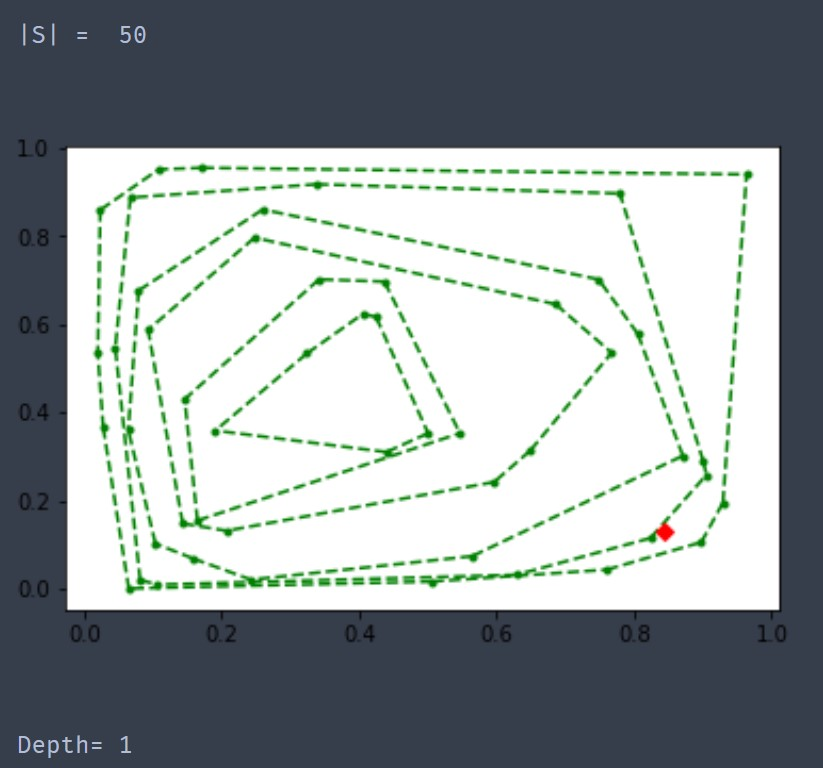
\includegraphics[scale=.1]{50_1.jpg}
			\label{fig:1}
		}
	}%\hspace{2cm}
	\subfigure[$|S|=50,\ depth=2$]{
		\resizebox{!}{3cm}{
			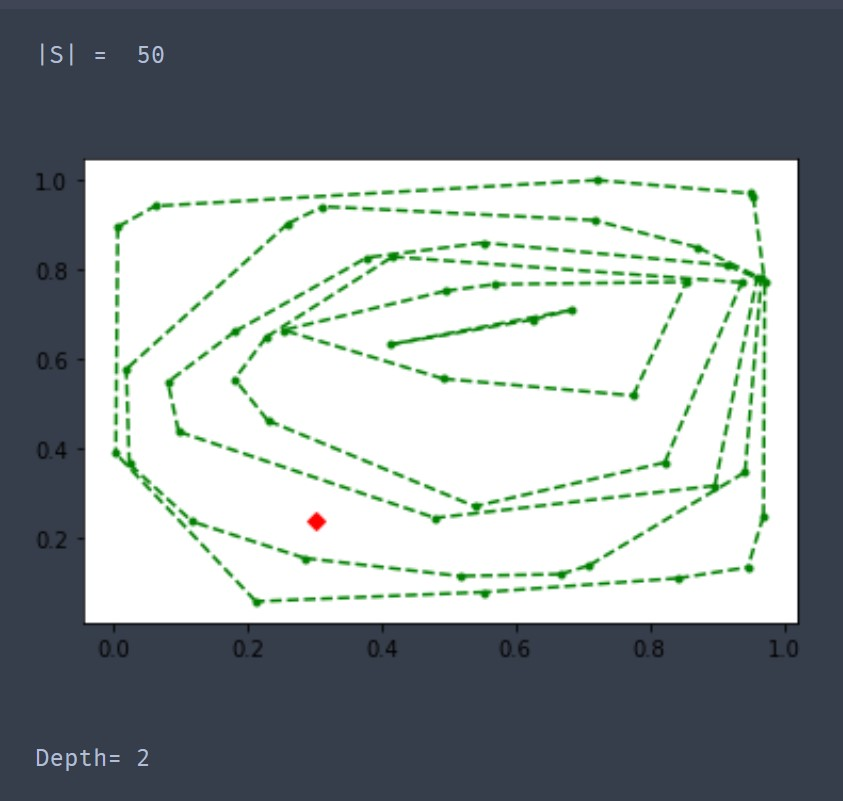
\includegraphics[scale=.1]{50_2.jpg}
			\label{fig:2}
		}
	}%\hspace{2cm}
	\subfigure[$|S|=50,\ depth=3$]{
		\resizebox{!}{3cm}{
			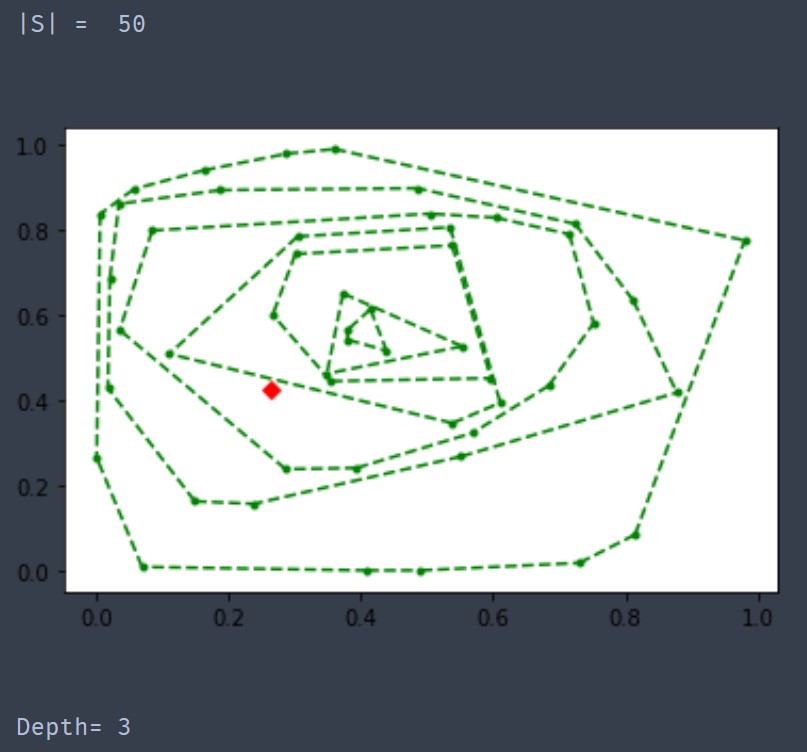
\includegraphics[scale=.1]{50_3.jpg}
			\label{fig:3}
		}
	}

	\subfigure[$|S|=100,\ depth=3$]{
		\resizebox{!}{4cm}{
			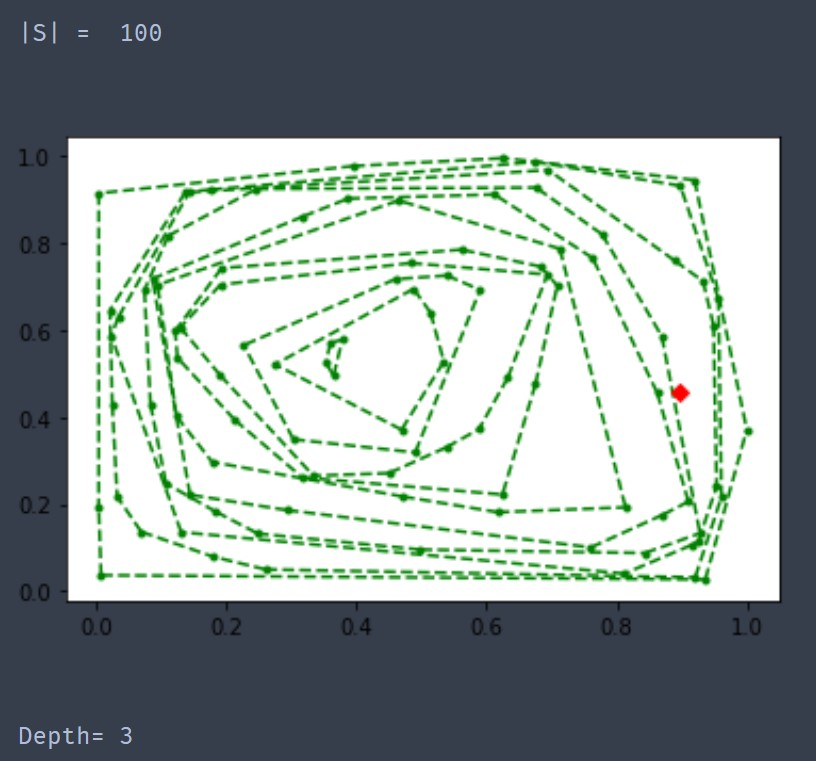
\includegraphics[scale=.1]{100_3.jpg}
			\label{fig:1}
		}
	}%\hspace{2cm}
	\subfigure[$|S|=100,\ depth=7$]{
		\resizebox{!}{4cm}{
			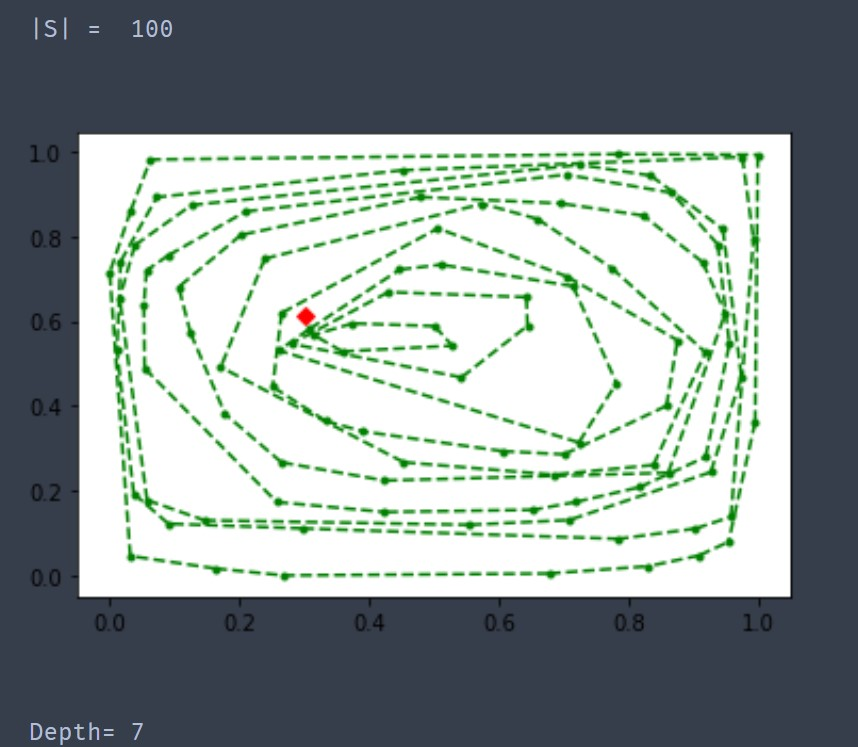
\includegraphics[scale=.1]{100_7.jpg}
			\label{fig:2}
		}
	}%\hspace{2cm}
	\subfigure[$|S|=100,\ depth=10$]{
		\resizebox{!}{4cm}{
			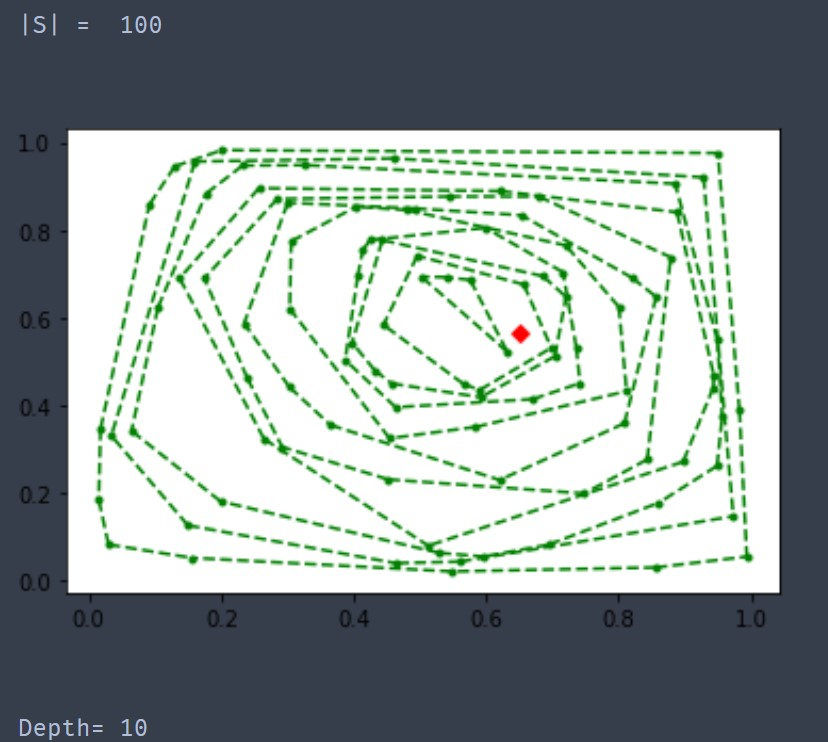
\includegraphics[scale=.1]{100_10.jpg}
			\label{fig:3}
		}
	}

	\subfigure[$|S|=200,\ depth=0$]{
		\resizebox{!}{4cm}{
			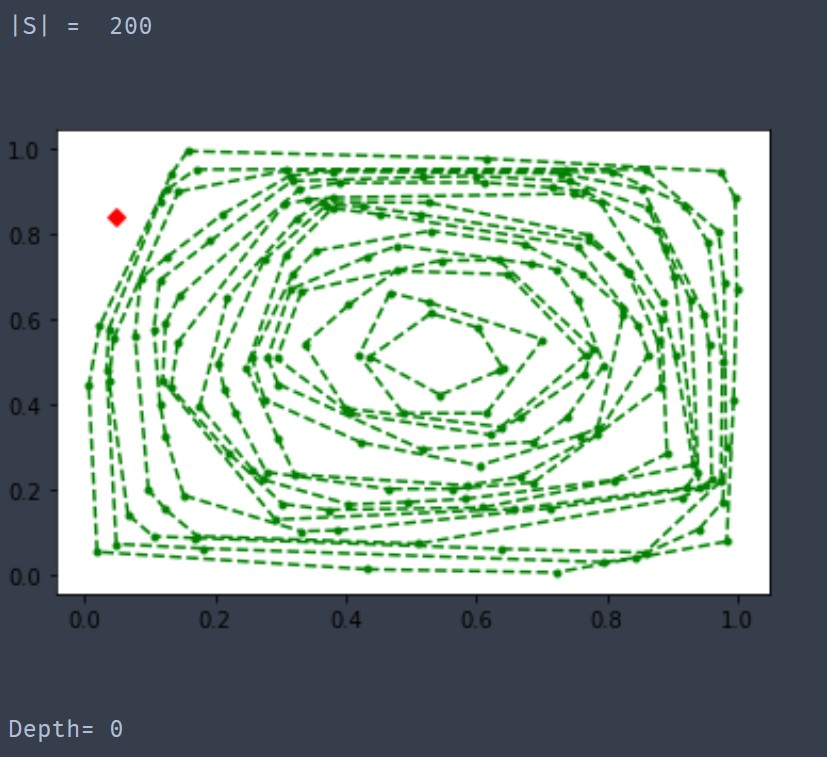
\includegraphics[scale=.1]{200_0.jpg}
			\label{fig:1}
		}
	}%\hspace{2cm}
	\subfigure[$|S|=200,\ depth=4$]{
		\resizebox{!}{4cm}{
			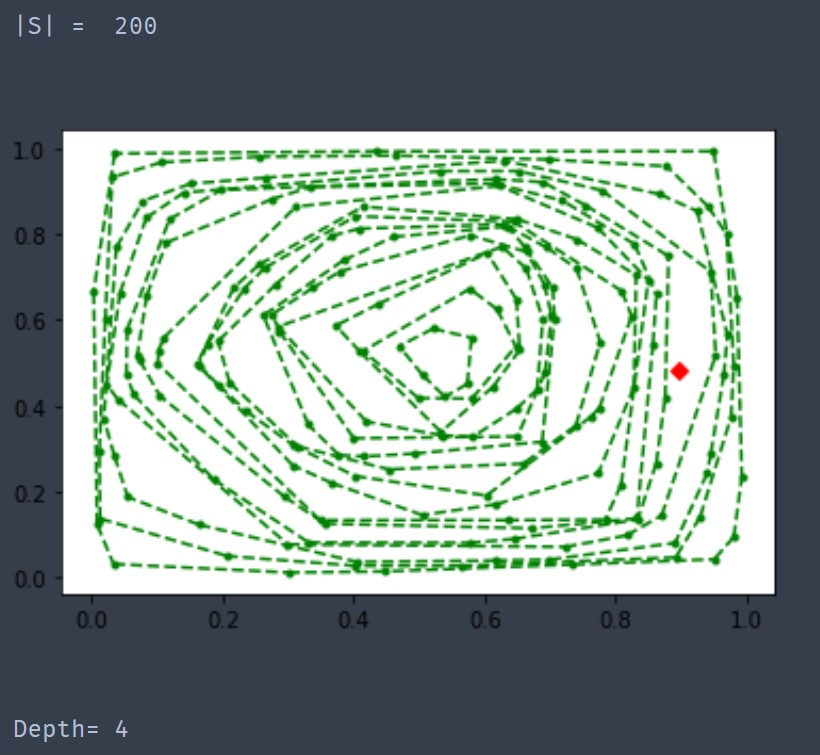
\includegraphics[scale=.1]{200_4.jpg}
			\label{fig:2}
		}
	}%\hspace{2cm}
	\subfigure[$|S|=200,\ depth=11$]{
		\resizebox{!}{4cm}{
			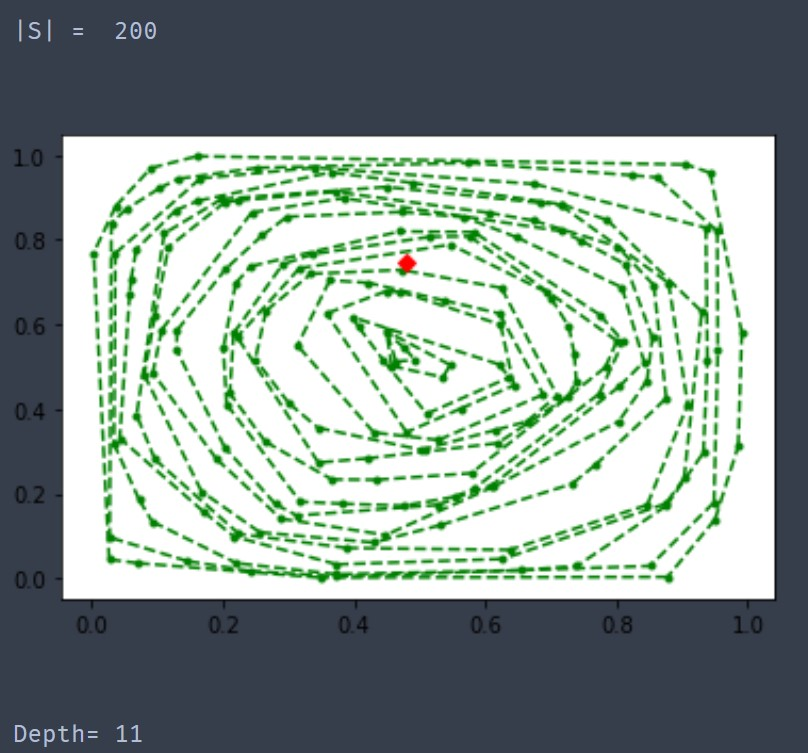
\includegraphics[scale=.1]{200_11.jpg}
			\label{fig:3}
		}
	}
	\caption{Runs of \Cref{alg:iterjarvis} with $|S|\in \{50,\ 100,\ 200\}.$ Red Point denotes the query point.}
	\label{fig:gen2}
\end{figure}
